\documentclass{beamer}
\usepackage[utf8]{inputenc}

\usetheme{Madrid}
\usecolortheme{default}
\usepackage{amsmath,amssymb,amsfonts,amsthm}
\usepackage{txfonts}
\usepackage{tkz-euclide}
\usepackage{listings}
\usepackage{adjustbox}
\usepackage{array}
\usepackage{tabularx}
\usepackage{gvv}
\usepackage{lmodern}
\usepackage{circuitikz}
\usepackage{tikz}
\usepackage{graphicx}

\setbeamertemplate{page number in head/foot}[totalframumber]

\usepackage{tcolorbox}
\tcbuselibrary{minted,breakable,xparse,skins}



\definecolor{bg}{gray}{0.95}
\DeclareTCBListing{mintedbox}{O{}m!O{}}{%
  breakable=true,
  listing engine=minted,
  listing only,
  minted language=#2,
  minted style=default,
  minted options={%
    linenos,
    gobble=0,
    breaklines=true,
    breakafter=,,
    fontsize=\small,
    numbersep=8pt,
    #1},
  boxsep=0pt,
  left skip=0pt,
  right skip=0pt,
  left=25pt,
  right=0pt,
  top=3pt,
  bottom=3pt,
  arc=5pt,
  leftrule=0pt,
  rightrule=0pt,
  bottomrule=2pt,
  toprule=2pt,
  colback=bg,
  colframe=orange!70,
  enhanced,
  overlay={%
    \begin{tcbclipinterior}
    \fill[orange!20!white] (frame.south west) rectangle ([xshift=20pt]frame.north west);
    \end{tcbclipinterior}},
  #3,
}
\lstset{
    language=C,
    basicstyle=\ttfamily\small,
    keywordstyle=\color{blue},
    stringstyle=\color{orange},
    commentstyle=\color{green!60!black},
    numbers=left,
    numberstyle=\tiny\color{gray},
    breaklines=true,
    showstringspaces=false,
}
%------------------------------------------------------------
%This block of code defines the information to appear in the
%Title page
\title %optional
{2.7.14}
\date{September 17,2025}
%\subtitle{A short story}

\author % (optional)
{EE25BTECH11002 - Achat Parth Kalpesh}



\begin{document}

\frame{\titlepage}

\begin{frame}{Question}
If $\theta$ is the angle between the two vectors $\vec{a} = \hat{i} - 2\hat{j} + 3\hat{k}$ and $\vec{b} = 3\hat{i} - 2\hat{j} + \hat{k}$, find $\sin \theta$.
\end{frame}

\begin{frame}{Theoretical Solution}
Let the given vectors be represented by column matrices $\vec{a}$ and $\vec{b}$.
\begin{align}
    \vec{a} = \myvec{1 \\ -2 \\ 3}, \quad \vec{b} = \myvec{3 \\ -2 \\ 1}
\end{align}
The sine of the angle $\theta$ between two vectors is given by the formula:
\begin{align}
\sin\theta &= \sin\brak{\cos^{-1}\brak{\frac{\abs{\vec{a}^\top\vec{b}}}{\norm{\vec{a}} \norm{\vec{b}}}}}
\end{align}
\end{frame}

\begin{frame}{Theoretical Solution}
\begin{align}
  \sin\theta &= \sin\brak{\cos^{-1}\brak{\frac{\abs{\myvec{1&-2&3}\myvec{3\\-2\\1}}}{\norm{\myvec{1\\-2\\3}}\norm{\myvec{3\\-2\\1}}}}}\\
  &= \sin\brak{\cos^{-1} \brak{\frac{\abs{\brak{3}\brak{1} + \brak{-2}\brak{-2} + \brak{3}\brak{1}}}{\sqrt{1^2 + \brak{-2}^2 + 3^2}\sqrt{3^2 + \brak{-2}^2 + 1^2}}}}
\end{align}
\end{frame}

\begin{frame}{Theoretical Solution}
\begin{align}
   &= \sin\brak{\cos^{-1}\brak{\frac{\abs{3+4+3}}{\sqrt{14}\sqrt{14}}}}\\
    &= \sin\brak{\cos^{-1}\brak{\frac{10}{14}}}\\
    &= \frac{2\sqrt{6}}{7}
\end{align}
Therefore, the value of $\sin \theta$ is $\frac{2\sqrt{6}}{7}$.
\end{frame}

\begin{frame}[fragile]
    \frametitle{C code}
    \begin{lstlisting}
#include <stdio.h>
#include <math.h>
float formula(float *a,float *b)
{
    float c[3];
    c[0] = a[1]*b[2] - a[2]*b[1];
    c[1] = a[2]*b[0] - a[0]*b[2];
    c[2] = a[0]*b[1] - a[1]*b[0];
    
    return sqrt((c[0]*c[0] + c[1]*c[1] + c[2]*c[2]))/(sqrt(a[0]*a[0] + a[1]*a[1] + a[2]*a[2])*sqrt(b[0]*b[0] + b[1]*b[1] + b[2]*b[2]));
}
    \end{lstlisting}
\end{frame}

\begin{frame}[fragile]
    \frametitle{Python Code}
    \begin{lstlisting}[language=Python]
import numpy as np
import matplotlib.pyplot as plt
import ctypes
import os
import sys

# Load the shared C library
lib_path = ctypes.CDLL("./formula.so")

# Define the argument types for the C function
lib_path.formula.argtypes = [
    ctypes.POINTER(ctypes.c_float),
    ctypes.POINTER(ctypes.c_float)
]
# Define the return type for the C function
lib_path.formula.restype = ctypes.c_float
    \end{lstlisting}
\end{frame}

\begin{frame}[fragile]
    \frametitle{Python Code}
    \begin{lstlisting}[language=Python]
# Define the input vectors as numpy arrays
vecA = np.array([1, -2, 3], dtype=np.float32)
vecB = np.array([3, -2, 1], dtype=np.float32)

# Call the C function
sin_theta = lib_path.formula(
    vecA.ctypes.data_as(ctypes.POINTER(ctypes.c_float)),
    vecB.ctypes.data_as(ctypes.POINTER(ctypes.c_float))
)

print(f"The value of sin(theta) is: {sin_theta}")
# Theoretical value: 2*sqrt(6)/7 = 0.700
    \end{lstlisting}
\end{frame}

\begin{frame}[fragile]
    \frametitle{Python Code: Plotting}
    \begin{lstlisting}[language=Python]
# Create a 3D plot
fig = plt.figure(figsize=(8, 8))
ax = fig.add_subplot(111, projection='3d')

# Define the origin point
origin = np.array([0, 0, 0])

# Plot the two vectors from the origin using ax.quiver
ax.quiver(*origin, *vecA, color='blue', label='Vector a = (1, -2, 3)')
ax.quiver(*origin, *vecB, color='green', label='Vector b = (3, -2, 1)')

# Set the limits of the plot for better visualization
max_val = np.max(np.abs(np.concatenate((vecA, vecB)))) + 1
ax.set_xlim([-max_val, max_val])
ax.set_ylim([-max_val, max_val])
ax.set_zlim([-max_val, max_val])
    \end{lstlisting}
\end{frame}

\begin{frame}[fragile]
    \frametitle{Python Code: Finalizing Plot}
    \begin{lstlisting}[language=Python]
# Add labels and a title
ax.set_xlabel('X-axis')
ax.set_ylabel('Y-axis')
ax.set_zlabel('Z-axis')
ax.set_title('Two 3D Vectors')

# Add a legend
ax.legend()

# Add a grid for better visualization
ax.grid(True)

# Save and show the plot
plt.savefig("plot_c.jpg")
plt.show()
    \end{lstlisting}
\end{frame}

\begin{frame}{Plot}
    \begin{figure}
        \centering
        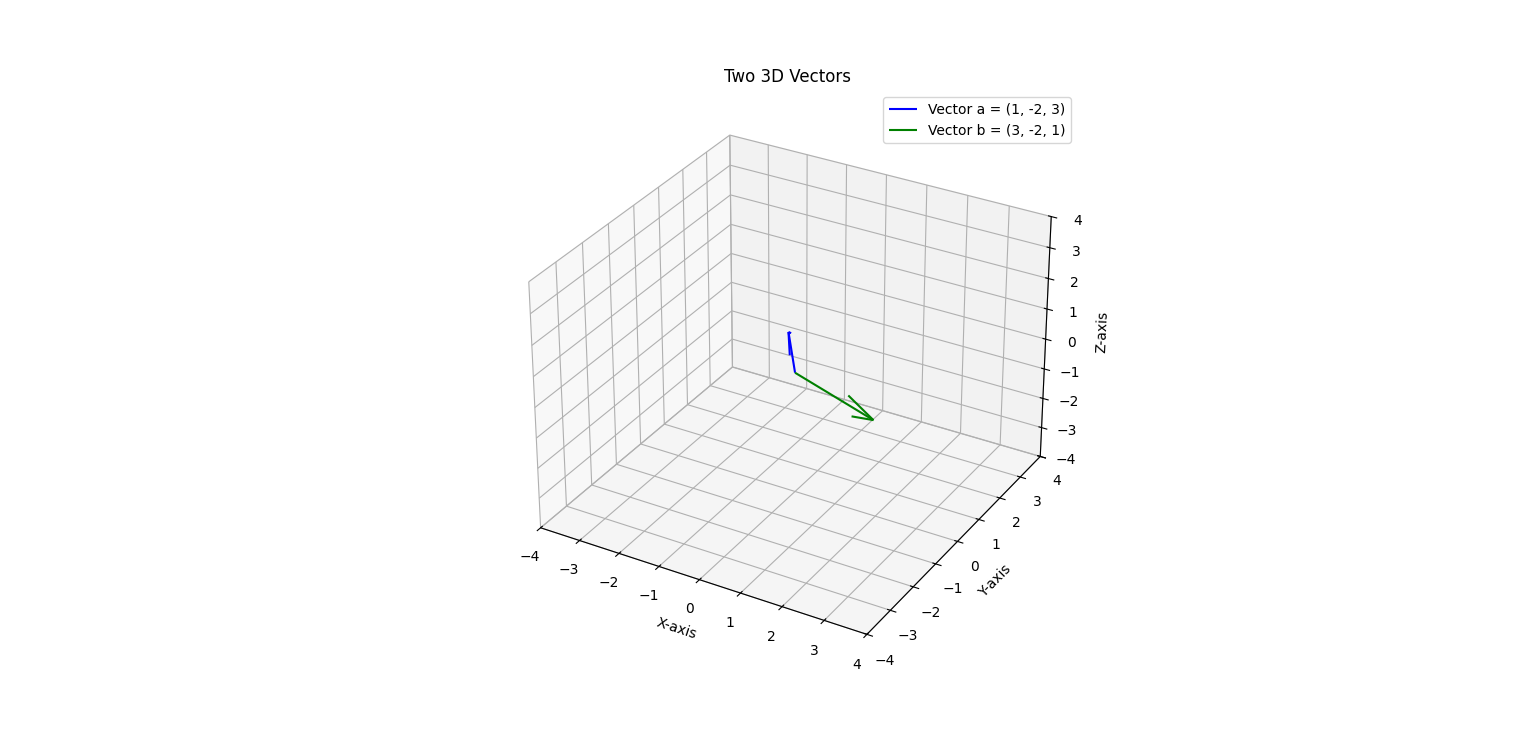
\includegraphics[width=0.9\columnwidth]{../figs/pure_python.png}
        \caption{Visualization of the two vectors}
        \label{fig:final_plot}
    \end{figure}
\end{frame}

\end{document}
